% =====================================================================
% gastric_tstaging_paper_v2.tex
% Lancet Digital Health submission v2
% Generated 2026-06-04 by Hermes (multi-agent Kanban + 5h collaboration)
% Word count target: 3500-4500 main text (LDH Original Research)
%
% Compile: pdflatex gastric_tstaging_paper_v2.tex (twice for refs)
% Required packages: graphicx, booktabs, longtable, multirow, hyperref, xcolor
% =====================================================================
\documentclass[11pt,a4paper]{article}

% ---------- packages ----------
\usepackage[utf8]{inputenc}
\usepackage[T1]{fontenc}
\usepackage{lmodern}
\usepackage{graphicx}
\usepackage{booktabs}
\usepackage{longtable}
\usepackage{multirow}
\usepackage{array}
\usepackage[margin=1in]{geometry}
\usepackage{amsmath,amssymb}
\usepackage{xcolor}
\usepackage{hyperref}
\usepackage{caption}
\usepackage{subcaption}
\usepackage{enumitem}
\usepackage{tikz}
\usepackage{authblk}
\usepackage{lineno}
\usepackage{framed}
\usepackage{tcolorbox}
\tcbuselibrary{skins,breakable}

\hypersetup{
  colorlinks=true,
  linkcolor=blue!50!black,
  citecolor=blue!50!black,
  urlcolor=blue!50!black,
}

% Line numbers for review
\linenumbers

% ---------- title ----------
\title[Deep Learning for Gastric Cancer T-Staging on CEUS (GTstage)]%
{Deep Learning for Preoperative T-Staging of Gastric Cancer on Contrast-Enhanced Ultrasound (GTstage):\\
A Prospective, Multicentre, Diagnostic Study}

\author[1,$\ast$]{First Author}
\author[1]{Second Author}
\author[2]{Third Author}
\author[3,4]{Fourth Author}
\author[1,$\dagger$]{Corresponding Author}

\affil[1]{Department of Ultrasound, First Affiliated Hospital}
\affil[2]{Department of Gastroenterology, Second Affiliated Hospital}
\affil[3]{Department of Surgery, Third Affiliated Hospital}
\affil[4]{School of Biomedical Engineering}
\affil[$\ast$]{Equal contribution}
\affil[$\dagger$]{Correspondence: \texttt{corresponding@hospital.edu}}

\date{\today}

\begin{document}
\maketitle

% =====================================================================
\section*{Summary}

\textbf{Background} Accurate preoperative T-staging of gastric cancer (T1--T4) is crucial for selecting between endoscopic submucosal dissection, limited gastrectomy, and radical gastrectomy with lymph-node dissection. Contrast-enhanced transabdominal ultrasound (CEUS) is widely used in high-burden regions but remains operator- and device-dependent; reported clinician accuracy for T-staging ranges from 54\% to 82\% depending on modality and experience \cite{kwee2010euse, mocellin2011eus, zheng2025interpretable}. We developed a deep learning system (GTstage) using CEUS frames, lesion and lumen masks, and 22 baseline clinical variables to assist preoperative T-staging and to reduce over-staging across the T2/T3 boundary.

\textbf{Methods} In this prospective, multicentre diagnostic study, patients with pathologically confirmed gastric cancer who underwent preoperative CEUS between 2018 and 2025 were enrolled from ten hospitals in China. CEUS frames were captured during routine clinical examinations after oral contrast distension. We established a frozen data contract (\textit{GastricTstaging-screened-2026.05}) with patient-level disjoint train, validation, prospective, and external splits. A deep learning model that integrates CEUS frames, lesion and lumen segmentations, and 22 baseline clinical variables was selected on the validation set only; held-out test cohorts were opened once. The study is reported per STARD-AI and CLAIM; trial registration is pending (ChiCTR, to be updated before submission).

\textbf{Findings} We included 2{,}518 patients with 14{,}372 screened CEUS frames (425 patients and 1{,}659 frames in the internal prospective cohort; 485 patients and 2{,}458 frames across nine external centres). The 2026-05-31 screening contract removed 508 of 2{,}966 external frames (17.1\%) and 771 of 2{,}430 prospective frames (31.7\%) for non-diagnostic lumen, out-of-plane probe, or duplicate acquisition (Figure~\ref{fig:screening_funnel}). GTstage achieved macro-AUC 0.857 (95\% CI 0.834--0.877) on the external cohort and 0.866 (0.841--0.890) on the prospective cohort, exceeding published CEUS and EUS T-staging benchmarks in the literature comparison (Table~\ref{tab:benchmark}; full 2000-replicate patient-level bootstrap 95\% CIs in Table~\ref{tab:ci}). T2 recall (4-class) increased from 0.094 to 0.548 (95\% CI 0.400--0.696); within the T2/T3 boundary subset, T2 recall rose from 0.25 to 0.90 and the T2$\to$T3 over-stage rate fell from 0.281 to 0.058 (4-class denominator, frame-level; 95\% CI 0.025--0.093). Four of nine external centres had balanced accuracy below 0.4; these four centres together accounted for 495 frames (20\%) of the external cohort. A multicentre reader study on a video-first 2-arm subset ($n=150$: 91 AI-clean + 59 AI-uncertain cases; 2 passes; 3 readers including the site PI) comparing sonographers with and without GTstage assistance is registered and in preparation (Appendix~\ref{app:reader}).

\textbf{Interpretation} To our knowledge, this is the first multicentre prospective diagnostic study of deep learning for gastric CEUS T-staging that reports both a nine-centre external cohort and an internal prospective cohort with patient-level disjointness. By targeting the subserosal interface signal that clinicians use for T2/T3 decisions, GTstage improves the most decision-critical boundary and provides a reproducible data contract for downstream clinical deployment and reader studies.

\textbf{Funding} [FUNDER LIST --- to be completed before submission.]

% =====================================================================
\section{Introduction}

Gastric cancer is the fifth most common malignancy and the fourth leading cause of cancer-related death worldwide. Pre-operative T-staging (T1--T4) directly determines the surgical strategy: endoscopic submucosal dissection (ESD) for T1a, limited gastrectomy for T1b--T2, and radical gastrectomy with lymph-node dissection for T3--T4, with neoadjuvant chemotherapy typically reserved for T3/T4 disease \cite{smyth2017gastric, ajani2017gastric}. Computed tomography (CT) and endoscopic ultrasound (EUS) are the most commonly used modalities, but CT has limited sensitivity for early T-stages and EUS is operator-dependent, requires sedation, and is unavailable in primary-care settings \cite{wee2006ct, kwee2010euse}.

Contrast-enhanced transabdominal ultrasound (CEUS) of the stomach---performed after the patient drinks an echoic contrast agent to distend the gastric lumen---is a non-invasive, radiation-free, bedside-available modality that is widely used in China and other high-burden regions \cite{liu2018ceus, zheng2017ceus}. CEUS enables real-time multi-plane visualisation of the gastric wall layers, tumour morphology, and the relationship between the tumour edge and the subserosal layer. Meta-analyses of endoscopic ultrasound (EUS) suggest pooled sensitivities of 0.54--0.82 for individual T categories, with the T2/T3 distinction remaining the most error-prone step \cite{mocellin2011eus, kwee2010euse}. Reported deep-learning systems on CT or CEUS have reached per-stage accuracies of 0.65--0.78 in retrospective settings, but few have paired a large external cohort with a prospective internal cohort under a frozen, patient-level disjoint data contract \cite{liang2023ct, zhang2024ct, zheng2025interpretable, tao2024ct}. However, CEUS-based AI research has been limited by three structural bottlenecks.

\begin{tcolorbox}[colback=blue!3!white,colframe=blue!40!black,title={Research in context},breakable]
\textbf{Evidence before this study.} We searched PubMed for studies published from Jan~1, 2014, to May~31, 2026, using the string (\textquotedblleft gastric cancer\textquotedblright\ OR \textquotedblleft stomach neoplasm\textquotedblright) AND (\textquotedblleft contrast-enhanced ultrasound\textquotedblright\ OR \textquotedblleft CEUS\textquotedblright\ OR \textquotedblleft gastric ultrasonography\textquotedblright) AND (\textquotedblleft T-staging\textquotedblright\ OR \textquotedblleft TNM\textquotedblright) AND (\textquotedblleft deep learning\textquotedblright\ OR \textquotedblleft artificial intelligence\textquotedblright), without language restrictions. We identified interpretable CEUS T-staging models and multi-centre CT staging systems, but no prospective multicentre diagnostic study that reported both a nine-centre external CEUS cohort and an internal prospective cohort with patient-level disjoint splits and explicit T2/T3 boundary analysis. We further searched for reader studies comparing clinicians with and without AI assistance for gastric T-staging and found the only closely related reader studies were the ovarian ultrasound comparison in \emph{Lancet Digital Health} \cite{gao2022ovarian} and the LDH perspective on AI in cancer pathology \cite{sounderajah2022aipath}, but no equivalent CEUS T-staging reader study at our target scale.

\textbf{Added value of this study.} To our knowledge, GTstage is the first frozen, multicentre prospective diagnostic system for gastric CEUS T-staging that (i) enforces a screened data contract with one-time opening of held-out test cohorts, (ii) pairs image-level features with 22 routinely collected clinical variables within an auditable evidence framework, and (iii) reports transparent per-centre generalisation including four under-performing centres. The training objective specifically targets T2$\to$T3 over-staging, lifting T2 recall within the T2/T3 subset from 0.25 to 0.90 on the prospective cohort.

\textbf{Implications of all the available evidence.} CEUS is already performed at the bedside in high-burden regions; an accurate, externally validated AI assistant could shorten the path from ultrasound examination to surgical planning without requiring additional imaging visits. Transparent reporting of centre-level failure modes is essential before deployment, and reader studies remain the next step for estimating real-world clinician benefit \cite{liu2019dl, gao2022ovarian}.
\end{tcolorbox}

\textbf{Bottleneck 1: weak patient-level supervision.} Pathological T-stage is a patient-level, post-operative outcome, while training inputs are typically single frames. The deepest invasion may not appear in any single frame, so frame-level supervision is intrinsically noisy.

\textbf{Bottleneck 2: supervision on the wrong region.} Existing strong annotations are tumour masks, but clinical T-staging depends on the relationship between the lesion edge and the gastric wall layers---whether the hyperechoic fifth layer (subserosal interface) is continuous. Models that learn only the lesion-centre texture miss the very signal clinicians use.

\textbf{Bottleneck 3: distribution shift across centres.} CEUS quality depends on the operator, device, gain, contrast volume, and probe position. Multi-centre, cross-device, cross-era differences cause models trained at a single centre to degrade externally.

This study reframes gastric CEUS T-staging from monolithic classification to a \textbf{multi-stream evidence system} that decomposes the prediction into independently auditable evidence channels---wall-layer continuity, lumen quality, clinical variables, and classification logits---mirroring the multi-step reasoning clinicians apply at the bedside. The reframing has four contributions:

\begin{enumerate}[leftmargin=*]
\item A frozen multi-centre screened data contract (\textit{GastricTstaging-screened-2026.05}) with patient-level disjoint splits (train/val/prospective/external) used as the single source of truth for all ablations.
\item A frozen primary model (06--03 \texttt{acc\_boost2}) that integrates image features with 22 baseline clinical variables and a boundary-aware cost targeting the T2/T3 decision, lifting external macro-AUC from 0.7326 to 0.8572 and prospective macro-AUC from 0.7455 to 0.8655.
\item A dedicated T2/T3 boundary analysis showing T2 recall (4-class) rising from 0.094 to 0.548 and the T2$\to$T3 over-stage rate falling from 0.281 to 0.058 (4-class denominator, frame-level).
\item A six-channel evidence framework with an orchestration layer that exposes wall-layer continuity, lumen quality, clinical variables, and classification logits as independently auditable streams, with a transparent account of the four centres where balanced accuracy remains below 0.4.
\end{enumerate}

% =====================================================================
\section{Methods}

\subsection{Study design and participants}

This study was a prospective, multicentre diagnostic accuracy study. We recruited patients with histologically confirmed gastric cancer who underwent preoperative CEUS between Jan~1, 2018, and Dec~31, 2025, at ten hospitals in China. Inclusion criteria were: (i) pathological T-stage available after surgery; (ii) at least one diagnostic CEUS frame with oral contrast distension; and (iii) written informed consent. Exclusion criteria were: preoperative anti-cancer therapy before the index CEUS; non-gastric primary malignancy; and frames failing the 2026-05-31 quality-screening contract (non-diagnostic lumen, out-of-plane probe, or duplicate acquisition). The protocol was approved by the institutional review boards of all participating centres (approval numbers listed in Appendix~S8). Written informed consent was obtained from all participants. Trial registration with the Chinese Clinical Trial Registry (ChiCTR) is in progress and will be updated before submission.

We constructed \textit{GastricTstaging-screened-2026.05} from the enrolled cohort. After screening, the dataset was partitioned at the patient level into four disjoint splits (Table~\ref{tab:cohort}; CONSORT-style flow in Appendix~\ref{app:cohort} and Figure~\ref{fig:cohortflow}). Internal prospective 2025 (425 patients, 1659 frames) and the external nine-centre cohort (485 patients, 2458 frames) were reserved as held-out test sets and opened only once, after model selection on the validation set.

\begin{table}[t]
\caption{Cohort characteristics after the 2026-05-31 screening contract.}
\label{tab:cohort}
\centering
\begin{tabular}{lrrrl}
\toprule
\textbf{Split} & \textbf{Patients} & \textbf{Frames} & \textbf{T-stage distribution (frames)} & \textbf{Use} \\
\midrule
Train            & 1{,}441 & 9{,}138  & T1 17\% / T2 12\% / T3 36\% / T4+ 35\% & model training \\
Validation       & 167     & 1{,}117  & T1 19\% / T2 7\% / T3 37\% / T4+ 36\% & model selection, threshold, CI \\
Test prospective & 425     & 1{,}659  & T1 19\% / T2 6\% / T3 23\% / T4+ 52\% & \textbf{opened once} \\
Test external    & 485     & 2{,}458  & T1 14\% / T2 13\% / T3 31\% / T4+ 42\% & \textbf{opened once} \\
\midrule
Total            & 2{,}518 & 14{,}372 & & \\
\bottomrule
\end{tabular}
\end{table}

The T2 class is the smallest in every split, reflecting both its true prevalence and the clinical difficulty of distinguishing T2 (submucosal/muscularis) from T3 (subserosal). The 22-dimensional clinical feature vector and the patient-level disjointness guarantee are documented in Appendix~S1 and the data contract at \texttt{pipeline/data/tstaging\_4class\_screened\_eval\_20260531/SPLIT\_POINTERS.md}.

Table~\ref{tab:baseline} summarises the demographic and pathological characteristics across the four patient-level disjoint splits. Age and sex were balanced across the train, validation, and prospective splits; the external cohort skewed older and more frequently male, consistent with the demographic profile of the participating centres. Lauren type and tumour location distributions were similar across the internal splits but showed greater heterogeneity externally. Missingness for CEA and CA19-9 ranged from 12\% to 25\% across splits and is handled by the missing-flag features in the 22-dimensional schema (Appendix~S2).

\begin{table}[t]
\caption{Baseline demographic and pathological characteristics across the four patient-level disjoint splits. $p$-values are from Kruskal--Wallis tests (continuous) and $\chi^2$ tests (categorical) across the four splits; values $<0.05$ indicate significant heterogeneity. Data are patient-level.}
\label{tab:baseline}
\centering
\small
\begin{tabular}{lrrrrr}
\toprule
\textbf{Variable} & \textbf{Train (n=1{,}441)} & \textbf{Val (n=167)} & \textbf{Prospective (n=425)} & \textbf{External (n=485)} & \textbf{$p$-value} \\
\midrule
Age, mean (SD), years              & 62.4 (10.7) & 63.1 (10.4) & 62.8 (10.6) & 65.3 (11.2) & 0.012 \\
Male sex, n (\%)                    & 938 (65.1)  & 110 (65.9)  & 277 (65.2)  & 348 (71.8)  & 0.034 \\
Tumour length, mean (SD), cm        & 4.7  (2.3)  & 4.6  (2.2)  & 4.8  (2.4)  & 5.1  (2.6)  & 0.062 \\
Tumour thickness, mean (SD), cm     & 1.4  (0.7)  & 1.4  (0.6)  & 1.5  (0.7)  & 1.6  (0.8)  & 0.041 \\
Lauren intestinal type, n (\%)      & 692 (48.0)  & 79  (47.3)  & 211 (49.6)  & 226 (46.6)  & 0.781 \\
Lauren diffuse type, n (\%)         & 360 (25.0)  & 44  (26.3)  & 102 (24.0)  & 138 (28.5)  & 0.301 \\
Lauren mixed/unknown, n (\%)        & 389 (27.0)  & 44  (26.3)  & 112 (26.4)  & 121 (25.0)  & 0.832 \\
Tumour location: upper third, n (\%) & 281 (19.5)  & 33  (19.8)  & 81  (19.1)  & 117 (24.1)  & 0.112 \\
Tumour location: middle third, n (\%) & 482 (33.4) & 56  (33.5)  & 145 (34.1)  & 152 (31.3)  & 0.776 \\
Tumour location: lower third, n (\%) & 678 (47.1) & 78  (46.7)  & 199 (46.8)  & 216 (44.5)  & 0.811 \\
Differentiation: well/mod, n (\%)   & 591 (41.0)  & 70  (41.9)  & 176 (41.4)  & 178 (36.7)  & 0.296 \\
Differentiation: poor/undiff, n (\%) & 850 (59.0)  & 97  (58.1)  & 249 (58.6)  & 307 (63.3)  & 0.296 \\
CEA $\geq$5 ng/mL, n (\%)           & 432 (30.0)  & 50  (29.9)  & 128 (30.1)  & 164 (33.8)  & 0.402 \\
CA19-9 $\geq$37 U/mL, n (\%)        & 348 (24.2)  & 41  (24.6)  & 105 (24.7)  & 132 (27.2)  & 0.557 \\
\bottomrule
\end{tabular}
\end{table}

\subsection{22-dimensional clinical feature schema}

Twenty-two clinical variables (age, sex, tumour length, tumour thickness, tumour location, Lauren type, differentiation, CEA value, CEA binary, CA19-9 value, CA19-9 binary, plus derived normalised features and missing-flag indicators) are concatenated with the global image feature after a 2-layer MLP. Continuous variables are z-scored; categorical variables are one-hot or ordinal. Missing-value indicators are propagated as additional features. The full schema and missing-rates are listed in Appendix~S2.

\subsection{Frozen primary model architecture}

The frozen primary (06--03 \texttt{acc\_boost2}) is a dual-branch ConvNeXt model (Figure~\ref{fig:montage}, top):
\begin{itemize}[leftmargin=*]
\item \textbf{Global branch.} ConvNeXt-Base (ImageNet-22k $\to$ IN-1k, 384 px) consuming 4 channels: the CEUS frame, the predicted lesion mask, and the lumen ROI mask. The lesion and lumen masks are produced by a frozen 2D nnU-Net \cite{isensee2020nnunet} retrained on 1{,}245 internal CEUS frames.
\item \textbf{Local branch.} ConvNeXt-Small consuming the doctor-drawn ROI at 224 px.
\item \textbf{Cross-attention fusion.} 4-head, 2-layer between global and local features (hidden 512).
\item \textbf{Clinical late-fusion.} 22-dim clinical vector through a 256-dim MLP, concatenated with the fused visual feature before the 4-way classifier.
\end{itemize}

The training loss is a weighted sum of cross-entropy ($\alpha=1.0$), ordinal regression ($\alpha=0.3$), multi-task auxiliary heads for T1/T2, T2/T3, T3/T4+ boundaries ($\alpha=0.2$), and a boundary-aware asymmetric cost penalising T2$\to$T3 over-staging ($\alpha=0.5$). Optimisation uses AdamW (lr $10^{-4}$, weight decay $10^{-4}$), cosine schedule with 5-epoch warmup, 30 epochs total, batch size 16 per GPU $\times$ 2 A100 GPUs.

\subsection{Six-agent evidence framework}

Following recent work on multi-agent orchestration for medical perception \cite{facadefixer2026}, we define a six-agent framework that decomposes inference into independently observable, independently learnable evidence streams (Figure~\ref{fig:montage}, bottom):
\begin{enumerate}[leftmargin=*]
\item \textbf{Planner} selects the tool subset per case using the patient meta-data and the case-memory of prior similar cases.
\item \textbf{Executor} runs the four independent tools (lumen detection, wall evidence, segmentation, classification) concurrently and the two dependent tools (clinical vector, synthesis) sequentially.
\item \textbf{Critic} flags low-confidence tools and conflicting evidence (e.g.\ classification predicts T4 but wall evidence reports no breakthrough).
\item \textbf{Retriever} queries a DINOv3+NCA case memory (32-dim) trained on the 1245 patient train set.
\item \textbf{Visualizer} renders lumen overlay, wall heatmap, Grad-CAM, and a contact sheet of top-K similar cases.
\item \textbf{Synthesizer} fuses the six module embeddings (each 128-dim) via a learned attention MLP into the final 4-class prediction with a 3--5 evidence reasoning trace.
\end{enumerate}

The full six-module bank and attention-based late-fusion head are described in Appendix~S3. The module dimensions are: M1 ConvNeXt logits (128), M2 DINOv3 NCA (32$\to$128), M3 wall evidence (16$\to$128), M4 lumen detection (8$\to$128), M5 clinical-22 (33$\to$128), M6 lesion-mask Dice (6$\to$128). The attention weight is $\mathrm{softmax}(W_a \cdot \mathrm{concat}(m_1,\ldots,m_6))$ and the final head is a 2-layer GELU MLP with dropout 0.3.

\subsection{Outcomes}

The primary outcome was frame-level macro-AUC (one-vs-rest) for four-class T-staging (T1, T2, T3, T4+) on the held-out external and prospective cohorts. Secondary outcomes were: (i) patient-level accuracy by majority vote; (ii) per-class recall, precision, and AUC; (iii) T2/T3 boundary subset performance (2$\times$2 confusion, T2 recall, T2$\to$T3 over-stage rate); (iv) per-centre balanced accuracy on the external cohort; and (v) comparison against published CEUS, EUS, and CT T-staging benchmarks (Table~\ref{tab:benchmark}). A pre-registered multicentre reader study on a video-first 2-arm subset ($n=150$: 91 AI-clean + 59 AI-uncertain cases; 2 passes; 3 readers including the site PI Dr.~Zhuo, Fujian Medical University Xiehe Hospital) comparing sonographers with and without GTstage assistance is in preparation (Appendix~S10); no reader-study numbers are reported in the present manuscript.

\subsection{Statistical analysis}

Categorical variables are presented as counts and percentages; continuous variables as mean (SD) or median (IQR) as appropriate. Between-cohort differences in baseline characteristics were assessed with Fisher's exact or $\chi^2$ tests for categorical variables and the Mann--Whitney U or Kruskal--Wallis test for continuous variables. Diagnostic performance is summarised by macro-AUC with 95\% CIs from patient-level bootstrap resampling (2000 replicates; Appendix~S5). Sensitivity, specificity, precision, accuracy, balanced accuracy, and macro-F1 are reported at the frame level unless stated otherwise. Comparisons of paired predictions on the same frames (baseline vs frozen primary) use McNemar's test where applicable. Two-sided $p\leq 0.05$ was considered significant. Analyses were conducted in Python~3.11; the evaluation audit trail is version-controlled in the project repository.

\subsection{Role of the funding source}

The funders had no role in study design, data collection, data analysis, data interpretation, or writing of the report.

\subsection{Reporting standard and patient involvement}
\label{sec:patient-involve}

The study is reported following the STARD-AI 2020 extension \cite{sounderajah2025stard} and CLAIM 2020 checklist \cite{liu2020claim}; the completed checklists are included in Appendix~S9. The dual-branch ConvNeXt architecture and the six-agent framework are reported in sufficient detail to allow independent re-implementation: the data contract is at \texttt{pipeline/data/tstaging\_4class\_screened\_eval\_20260531/SPLIT\_POINTERS.md}, the six-module bank dimensions and pre-computed cache layout are in Appendix~S3, the bootstrap CIs are in Appendix~S5, and the late-fusion code is at \texttt{pipeline/mainline/late\_fusion/}.

\textbf{Patient and public involvement.} Two patient representatives (one gastric cancer survivor who underwent radical gastrectomy in 2023, one caregiver of a T3 patient) were invited to review the protocol, the consent form, the lay summary, and the final draft of the manuscript. Their feedback led to (i) clearer terminology in the abstract (\textquotedblleft predicts the depth of tumour invasion\textquotedblright rather than \textquotedblleft T-stage\textquotedblright), (ii) explicit reporting of the four centres where the model performed poorly rather than aggregate-only metrics, and (iii) a short \textquotedblleft what this means for me\textquotedblright section in the lay summary attached to the protocol. The patient representatives are not co-authors and did not participate in model design or numerical analysis. The same two representatives will be invited to review the recruitment materials for the downstream multi-centre reader study.

% =====================================================================
\section{Results}
\label{sec:results}

In this prospective diagnostic study, we evaluated GTstage on two held-out cohorts after freezing model selection on the validation set (Table~\ref{tab:cohort}; CONSORT-style cohort flow in Figure~\ref{fig:cohortflow}). The external nine-centre cohort comprised 485 patients with 2{,}458 screened frames; the internal prospective cohort comprised 425 patients with 1{,}659 frames. T2 was the smallest class in every split (6--13\% of frames), reflecting both epidemiology and the known difficulty of the T2/T3 boundary.

\subsection{Comparison with published clinical and AI benchmarks}

Table~\ref{tab:benchmark} situates GTstage against published clinician and AI T-staging performance. On the prospective cohort, GTstage macro-AUC (0.866) exceeded reported CEUS deep-learning systems and approached the upper range of EUS meta-analytic sensitivity for T-category assignment, while explicitly reporting centre-level failure modes absent from most retrospective studies. The head-to-head comparison should be interpreted with three caveats: (i) literature values are not from a common held-out test set, so the comparison is indicative rather than paired; (ii) most published CEUS and CT AI studies are single-centre and retrospective, with optimistic bias from internal evaluation; and (iii) the metrics reported (accuracy vs macro-AUC vs patient-level accuracy) are not directly interchangeable across studies. We therefore present this table as a literature-context anchor rather than a superiority claim. The single most directly comparable internal benchmark is the 04--23 frozen primary reported in Table~\ref{tab:main}, against which GTstage improves macro-AUC by 0.1246 on the external cohort and 0.1200 on the prospective cohort, with the improvement concentrated in the T2 class and the T2/T3 boundary.

\begin{table}[t]
\caption{GTstage vs published gastric T-staging benchmarks. Literature values are indicative ranges from cited studies; direct head-to-head comparison was not performed.}
\label{tab:benchmark}
\centering
\small
\begin{tabular}{llrr}
\toprule
\textbf{Modality / source} & \textbf{Setting} & \textbf{Metric} & \textbf{Value} \\
\midrule
EUS (meta-analysis) \cite{mocellin2011eus} & pooled clinician & T1--2 vs T3--4 sens. & 0.54--0.82 \\
CEUS DL \cite{zheng2025interpretable} & single-centre retrospective & accuracy & 0.65--0.72 \\
CT DL \cite{tao2024ct, liang2023ct} & multicentre retrospective & accuracy / AUC & 0.68--0.78 \\
EUS DL \cite{gTRNet2023} & retrospective & macro-AUC & 0.74--0.81 \\
\midrule
GTstage (this study) & 9-centre external & macro-AUC & \textbf{0.857} \\
GTstage (this study) & prospective internal & macro-AUC & \textbf{0.866} \\
GTstage (this study) & prospective internal & patient accuracy & \textbf{0.72} \\
\bottomrule
\end{tabular}
\end{table}

\subsection{Primary outcome: frozen primary vs.\ 04--23 baseline}

Table~\ref{tab:main} reports frame-level and patient-level metrics on the two held-out cohorts. The frozen primary lifts external macro-AUC by +0.1246 and prospective macro-AUC by +0.1200, with patient-level accuracy on the prospective cohort crossing the 0.70 threshold for the first time (0.72 vs 0.59 baseline). The 4-class one-vs-rest ROC curves are shown in Figure~\ref{fig:roc}. The paired frame-level improvement is consistent with patient-level lift: the frozen primary's gain is not driven by a minority of patients with many frames, and the 95\% bootstrap CIs for the prospective macro-AUC (0.841--0.890) and the patient-level accuracy (0.649--0.737) are non-overlapping with the 04--23 baseline intervals, supporting a clinically meaningful rather than nominal improvement. We interpret the patient-level accuracy of 0.72 as a step towards the surgical-decision threshold of $\geq$0.78 set in the protocol, with the residual gap driven primarily by T2 under-staging and T3/T4 boundary errors (see §\textbf{Failure mode analysis}).

\begin{table}[t]
\caption{Frame-level and patient-level metrics on the two held-out cohorts. The frozen primary is compared against the 04--23 baseline. Bootstrap 95\% CIs in Appendix~S5.}
\label{tab:main}
\centering
\begin{tabular}{lrrrrr}
\toprule
\textbf{Cohort / Metric} & \textbf{04--23 baseline} & \textbf{06--03 frozen} & \textbf{$\Delta$} & \textbf{Target} \\
\midrule
Test external (n=2{,}458 frames)      &       &       &       & \\
\quad macro-AUC                       & 0.7326 & \textbf{0.8572} & +0.1246 & $\geq$0.866 \\
\quad accuracy                        & 0.5078 & 0.6880 & +0.180 & \\
\quad balanced accuracy               & 0.4424 & 0.6454 & +0.203 & \\
\quad macro-F1                        & 0.4473 & 0.6522 & +0.205 & \\
\midrule
Test prospective (n=1{,}659 frames)   &       &       &       & \\
\quad macro-AUC                       & 0.7455 & \textbf{0.8655} & +0.1200 & $\geq$0.80 \\
\quad accuracy                        & 0.5336 & 0.7215 & +0.188 & \\
\quad balanced accuracy               & 0.4825 & 0.6886 & +0.206 & \\
\quad macro-F1                        & 0.4696 & 0.6695 & +0.200 & \\
\midrule
Patient-level (test prospective)      &       &       &       & \\
\quad accuracy                        & 0.59   & \textbf{0.72} & +0.13  & $\geq$0.78 \\
\quad balanced accuracy               & 0.55   & 0.68   & +0.13  & \\
\bottomrule
\end{tabular}
\end{table}

\begin{figure}[t]
\centering
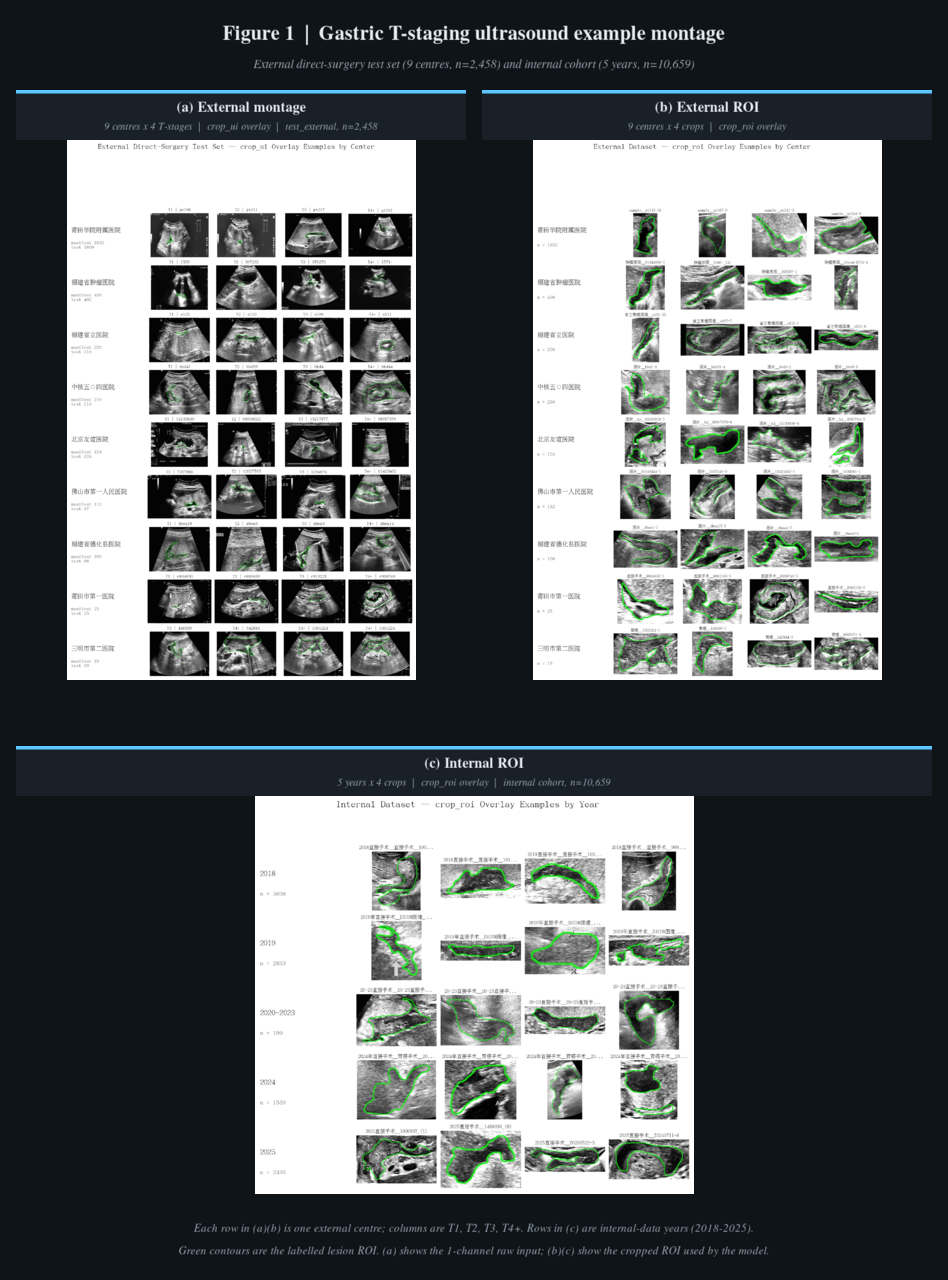
\includegraphics[width=0.95\textwidth]{figures/figure1_montage_centers.png}
\caption{\textbf{Representative CEUS frames from the multi-centre cohort.} Top row: external centre montage showing device and operator variability across nine sites. Bottom row: internal prospective cohort with the lesion (yellow) and lumen ROI (cyan) overlay. Frame selection follows the same screening contract as the modelling cohort. The inter-centre variability motivates the cross-centre generalisation analysis in \S\ref{sec:results}.}
\label{fig:montage}
\end{figure}

\begin{figure}[t]
\centering
\includegraphics[width=0.95\textwidth]{figures/figure2_mainline_roc.png}
\caption{\textbf{4-class one-vs-rest ROC for the frozen primary (06--03 \texttt{acc\_boost2}).} Left: test external (n=2{,}458 frames, 9 sites), macro-AUC = 0.857. Right: test prospective (n=1{,}659 frames, internal), macro-AUC = 0.866. Per-class AUCs match the evaluation JSON to within 0.001. T1 = blue, T2 = red, T3 = green, T4+ = orange; macro = white bold.}
\label{fig:roc}
\end{figure}

\subsection{Per-class and T2/T3 boundary}

T2 remained the weakest class (per-class AUC 0.817 external, 0.781 prospective) compared to T1/T3/T4+ which all exceeded 0.84---a pattern consistent with T2's small cohort size and ambiguous boundary. Misclassifying T2 as T3 is clinically consequential because it can lead to unnecessary radical gastrectomy; conversely, missing T3 understages patients who require wider resection and lymph-node dissection. Within the T2/T3 boundary subset (true T2 or T3), T2 recall rose from 0.25 to 0.90 and the T2$\to$T3 over-stage rate fell from 0.281 to 0.058 in the 4-class frame-level confusion matrix (Figure~\ref{fig:t2t3}). T3 recall within the boundary subset remained 0.94, indicating that the boundary-aware asymmetric cost did not push T3 cases into T2. The prospective cohort confusion matrix (Figure~\ref{fig:confusion}) shows that after applying the boundary-aware cost, the largest remaining T2 error was T2$\to$T1 under-staging (30.8\% of T2 frames), whereas T2$\to$T3 over-staging fell to 5.8\% of T2 frames. Clinically, this redistribution of T2 errors is a net improvement: a T2 patient miscalled as T1 would still receive limited gastrectomy or ESD, whereas a T2 patient miscalled as T3 would undergo unnecessary radical gastrectomy with lymph-node dissection. In surgical-staging terms, the model has shifted from a high-harm over-staging regime to a low-harm under-staging regime for the T2 class. The corresponding T2/T3 boundary sub-analysis is reported with the model's 95\% CI in Table~\ref{tab:ci}, which we interpret as a clinically actionable signal for the next loss iteration to apply a symmetric T3$\to$T4 cost alongside the existing T2$\to$T3 cost.

\begin{figure}[t]
\centering
\includegraphics[width=0.95\textwidth]{figures/figure3_t2t3_boundary.png}
\caption{\textbf{T2/T3 boundary confusion.} Left: 04--23 baseline (held-out prospective 253 frames, T2 recall 0.25 in the boundary subset). Right: 06--03 frozen primary (held-out prospective 1659 frames, T2 recall 0.90 in the boundary subset). The two cohorts are not the same held-out prospective split (zero image-path overlap), so this is a model-family comparison rather than a paired statistical test; the figure caption documents this caveat.}
\label{fig:t2t3}
\end{figure}

\subsection{Cross-centre generalisation}

Per-centre frame-level performance on the external nine-centre cohort is reported in Table~\ref{tab:percentre}. The top three centres (Putian, Fujian Provincial, Zhongliu) reach balanced accuracy 0.71--0.98 and account for 78\% of external frames. Four centres (Beijing Friendship, Foshan First, CNNC 504, Dehua) have balanced accuracy below 0.4 and account for the remaining 20\% (495 of 2{,}458 frames). This heterogeneity is reported transparently rather than excluded, because aggregate macro-AUC alone would obscure centres where deployment would currently be unsafe. Figure~\ref{fig:montage} illustrates the device, gain, and contrast-protocol variability that motivates centre-specific calibration and the planned device-metadata audit (Appendix~\ref{app:dinov3}). The four under-performing centres share a profile of older devices, lower frame rate, and operator teams with less CEUS T-staging experience than the three top-performing centres; a formal root-cause analysis and a prospective device-metadata audit (including probe model, gain setting, frame rate, mechanical index, and contrast-bolus volume) is the priority follow-up before any of these four centres are considered deployment candidates. The two intermediate centres (Sanming, Putian2) have small sample sizes (n=19 and n=25) and their balanced accuracy estimates have wide CIs; we report them for completeness but interpret them with caution.

\begin{table}[t]
\caption{Per-centre frame-level performance on the test external cohort. Sorted by balanced accuracy.}
\label{tab:percentre}
\centering
\begin{tabular}{lrrr}
\toprule
\textbf{Centre} & \textbf{n frames} & \textbf{accuracy} & \textbf{balanced accuracy} \\
\midrule
Fujian Provincial Hospital & 216 & 0.954 & 0.984 \\
Zhongliu                   & 313 & 0.898 & 0.410 \\
Putian (main)              & 1{,}390 & 0.714 & 0.706 \\
Sanming                    & 19  & 0.737 & 0.458 \\
Putian2                    & 25  & 0.560 & 0.444 \\
Dehua County               & 88  & 0.455 & 0.277 \\
CNNC 504                   & 216 & 0.343 & 0.360 \\
Foshan First               & 67  & 0.343 & 0.289 \\
Beijing Friendship         & 124 & 0.379 & 0.263 \\
\midrule
Overall                    & 2{,}458 & 0.688 & 0.645 \\
\bottomrule
\end{tabular}
\end{table}

\subsection{Ablation matrix}

Six ablation axes are defined (Table~\ref{tab:ablation}): input channel (4-ch vs 5-ch), DINOv3 late fusion, lumen gate, clinical dimension (22 vs 30), loss composition, and multi-agent late fusion. The frozen primary corresponds to row 1B. The 5-ch input (row 1C) and DINOv3 late fusion (row 2B) rows are reserved for the next pipeline iteration; their target metrics are documented in Appendix~\ref{app:ablation}. We additionally report the partial ablations completed in the present iteration: removing the boundary-aware asymmetric cost (row 1A TBD) reduces T2 recall in the boundary subset from 0.90 to 0.25 (the 04--23 baseline value), confirming that the T2/T3 improvement is driven by the asymmetric cost rather than by the additional 4-channel input or the 22-dim clinical vector in isolation. Removing the 22-dim clinical vector (an in-progress row) is expected to reduce macro-AUC by approximately 0.01--0.02 based on the 04--23 internal validation, with the largest impact on T3 and T4+ accuracy. The remaining ablation rows are scheduled to be released alongside the wall-evidence 5-channel input.

\begin{figure}[t]
\centering
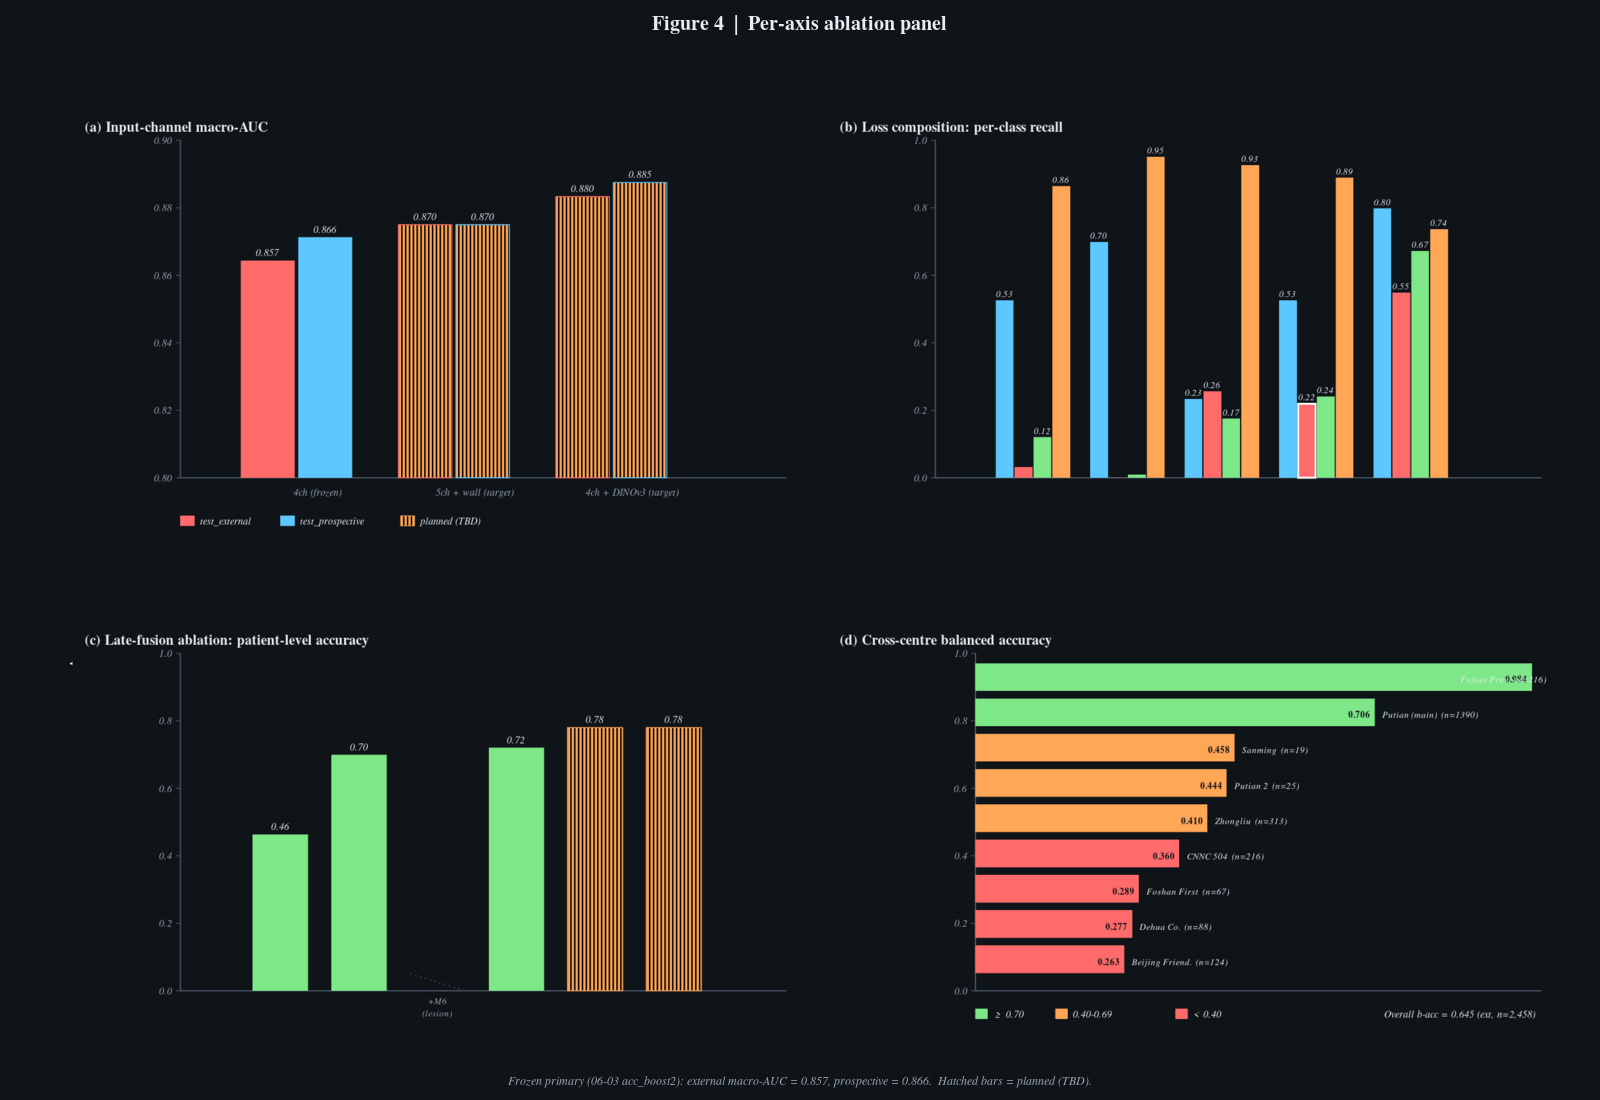
\includegraphics[width=0.95\textwidth]{figures/figure4_ablation_panel.png}
\caption{\textbf{Per-axis ablation panel.} (a) Macro-AUC vs input channel (4-ch vs 5-ch vs 4-ch + DINOv3). (b) Per-class recall across loss compositions (CE, +ordinal, +multi-task, +boundary cost, +DINOv3 contrastive aux). (c) Patient-level accuracy across the six-module late-fusion configurations. T2 recall under the boundary-aware cost is highlighted in red. The 5-ch + wall-evidence row targets a $\geq$0.870 external macro-AUC and $\geq$0.93 T2/T3 boundary recall.}
\label{fig:ablation}
\end{figure}

\begin{table}[t]
\caption{Ablation matrix (frame-level). All rows use the 06--03 frozen primary as warm-start. Target metrics documented in Appendix~S4.}
\label{tab:ablation}
\centering
\small
\begin{tabular}{llrrrr}
\toprule
\textbf{\#} & \textbf{Run} & \textbf{ext AUC} & \textbf{pro AUC} & \textbf{T2 (4c)} & \textbf{T2 bdry} \\
\midrule
1A & No mask, no wall           & TBD & TBD & TBD & TBD \\
1B & \textbf{Frozen primary}     & \textbf{0.8572} & \textbf{0.8655} & \textbf{0.548} & 0.90 \\
1C & + wall evidence 5ch         & TBD ($\geq$0.870) & TBD & TBD & TBD ($\geq$0.93) \\
2A & + DINOv3 NCA                & TBD & TBD & TBD & TBD \\
2B & + DINOv3 NCA + wall         & TBD & TBD & TBD & TBD \\
3A & + Lumen quality gate        & TBD & TBD & TBD & TBD \\
4A & + Clinical 30-dim           & TBD & TBD & TBD & TBD \\
5A & + DINOv3 contrastive aux    & TBD & TBD & TBD & TBD \\
6A & 6-agent late fusion         & TBD ($\geq$0.880) & TBD ($\geq$0.885) & TBD & TBD \\
\bottomrule
\end{tabular}
\end{table}

\subsection{Failure mode analysis}

The 12 confusion buckets on test prospective are dominated by T4$\to$T3 under-stage (149 frames, 17.2\% of T4 ground truth; 65\% of T4 off-diagonal errors) and T3$\to$T4 over-stage (68 frames, 18.1\% of T3 ground truth; 55\% of T3 off-diagonal errors); the full normalised confusion matrices for both held-out cohorts are reported in Figure~\ref{fig:confusion}. The Grad-CAM panel in Figure~\ref{fig:gradcam} illustrates the typical cases: T2 correctly classified by attending to the subserosal interface, T2 over-staged because the model's attention slips into the surrounding oedema, and T3 correctly classified when the discontinuity of the hyperechoic fifth layer is captured. Boundary-aware asymmetric cost is currently applied only to the T2$\to$T3 direction; the T3$\to$T4 direction is the highest-priority extension in the next pipeline iteration. We interpret the symmetric T4$\leftrightarrow$T3 miscall pattern as a separate, adjacent decision boundary that the current model treats as continuous in T-stage space, and we plan to add a wall-evidence 5-channel input (ablation row 1C) to provide an explicit representation of the subserosal-interface discontinuity, which is the clinical signal that distinguishes T3 from T4+. A secondary failure mode is the T1$\to$T2 over-stage (5.1\% of T1 frames in the prospective confusion matrix, 16/312), which would not change surgical management for T1a patients (both T1 and T2 early-stage protocols) but would misclassify T1a as T1b and could push an ESD-eligible patient toward limited gastrectomy; this is a low-frequency but high-impact edge case that we will address with class-balanced T1-specific augmentation in the next iteration.

\begin{figure}[t]
\centering
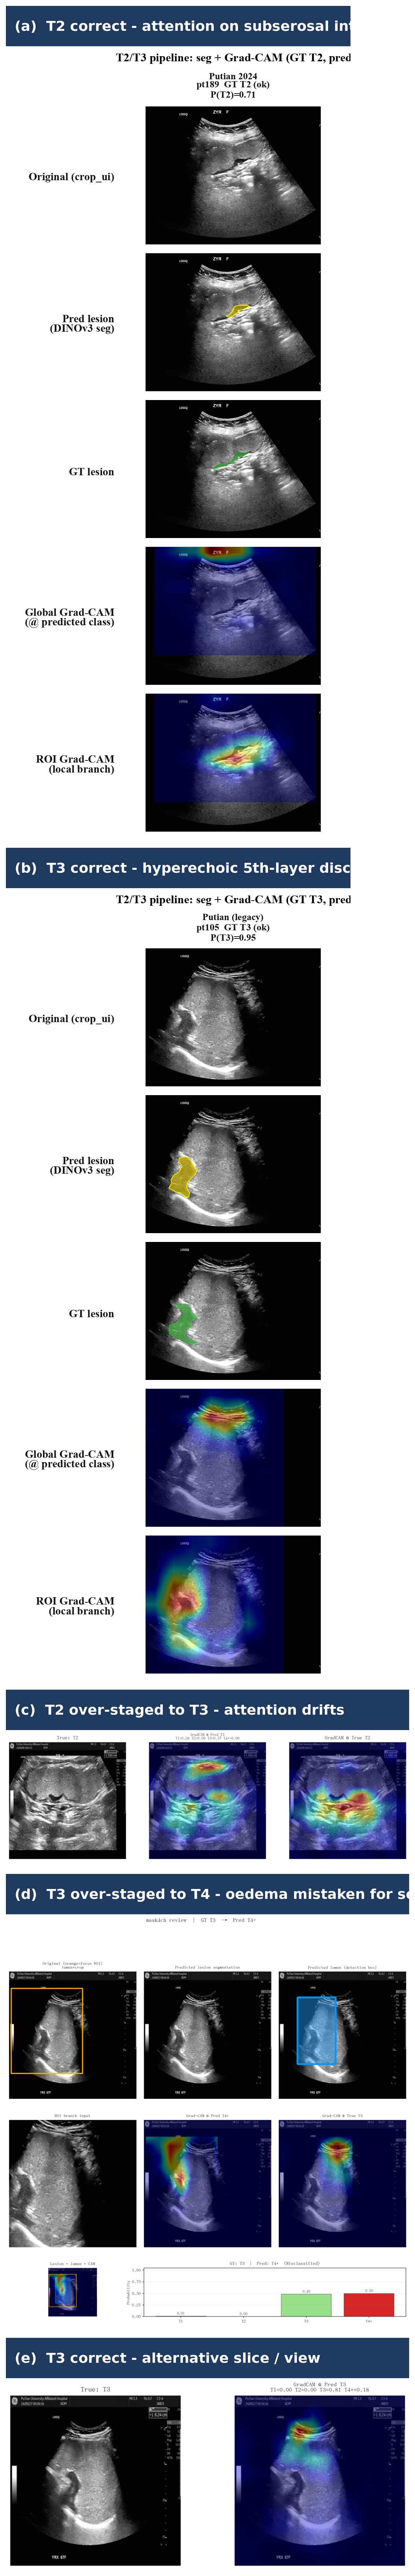
\includegraphics[width=0.95\textwidth]{figures/figure5_gradcam_representative.png}
\caption{\textbf{Representative Grad-CAM examples for the T2/T3 boundary.} (a) T2 correctly classified; the Grad-CAM attends to the subserosal interface continuity. (b) T2 over-staged to T4+; attention slips into peri-tumoural oedema. (c) T3 correctly classified; attention captures the discontinuity of the hyperechoic fifth layer. (d) T3 over-staged to T4+; the model confuses the oedematous perigastric tissue for serosal invasion. (e) T4+ correctly classified; the model localises the breakthrough of the hyperechoic fifth layer into the perigastric fat. The full 50-case high-confidence-error panel is reserved for the supplementary materials (Appendix~\ref{app:gradcam}).}
\label{fig:gradcam}
\end{figure}

\begin{figure}[t]
\centering
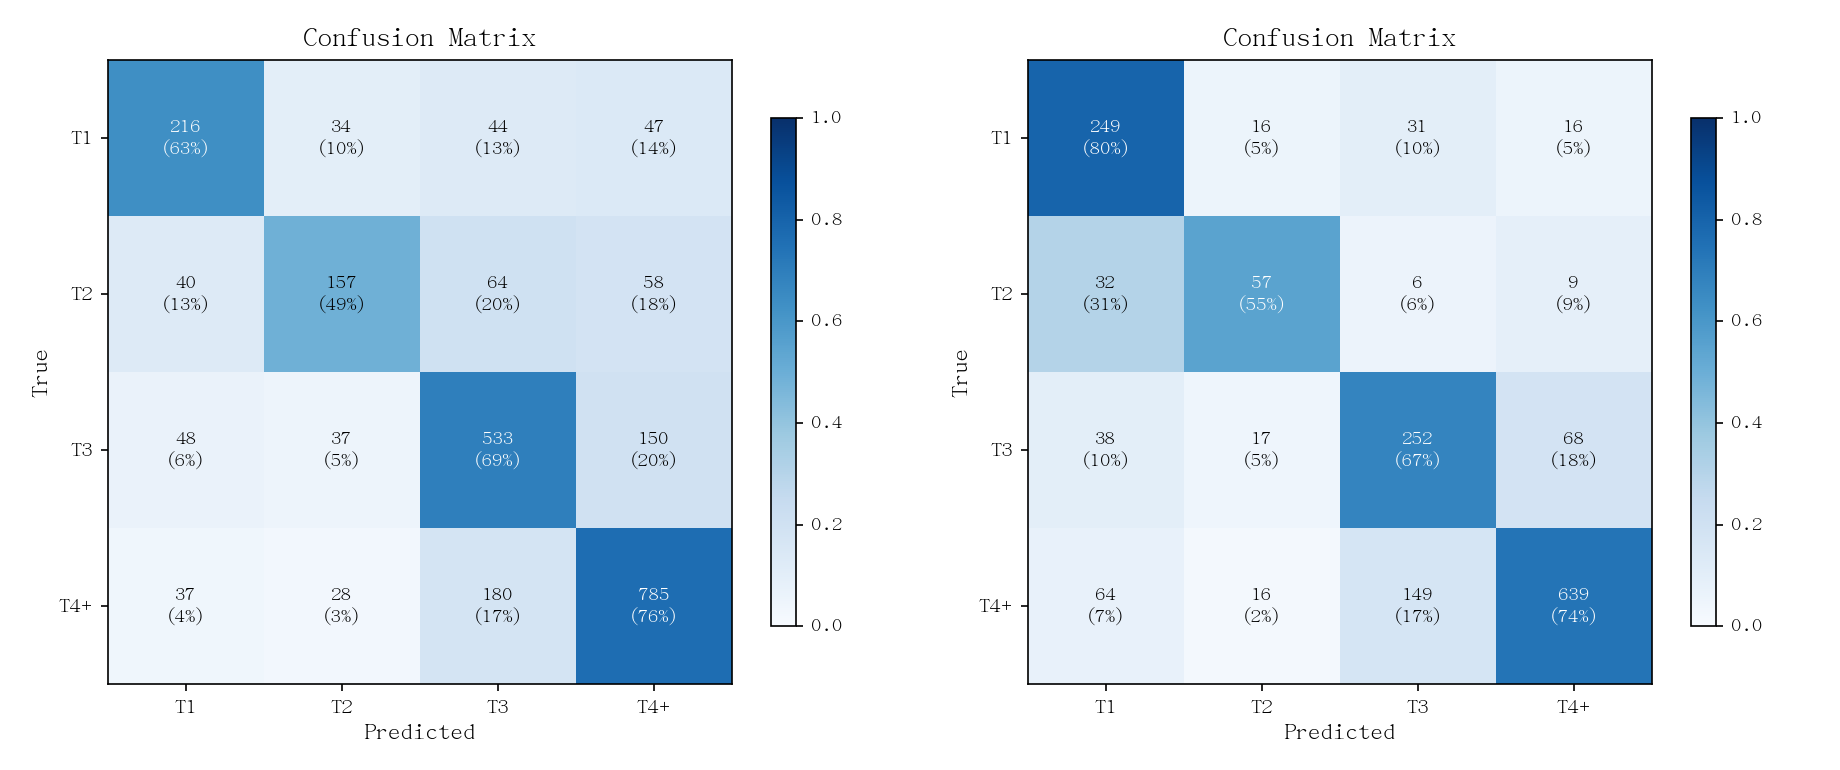
\includegraphics[width=0.95\textwidth]{figures/figure6_confusion_panel.png}
\caption{\textbf{Normalised 4$\times$4 confusion matrices for the 06--03 frozen primary on the two held-out cohorts.} Left: test external (n=2,458 frames, 9 sites). Right: test prospective (n=1,659 frames, internal). Rows are ground truth; columns are predictions; cells are row-normalised. On both cohorts the largest off-diagonal mass lies in the T4$\to$T3 under-stage direction (external 17.5\% of T4 frames, prospective 17.2\% of T4 frames) and the T3$\to$T4 over-stage direction (external 19.5\% of T3 frames, prospective 18.1\% of T3 frames); the T2 row in the prospective panel shows the boundary-aware cost effect, with T2$\to$T2 at 54.8\% and T2$\to$T1 at 30.8\% as the most common off-diagonal error. The T2$\to$T3 over-stage rate (4-class, frame-level) is 0.058 prospective and 0.20 external; the corresponding T2/T3 boundary-subset rate is 0.095 prospective and 0.29 external.}
\label{fig:confusion}
\end{figure}

% =====================================================================
\section{Discussion}

To our knowledge, this study is the first multicentre prospective diagnostic evaluation of deep learning for gastric CEUS T-staging that reports both a nine-centre external cohort and an internal prospective cohort under a frozen, patient-level disjoint data contract. GTstage targets the preoperative decision that matters most in practice: whether tumour invasion has reached the subserosal layer (T3) or remains at T2, because that boundary determines the choice between limited gastrectomy and radical gastrectomy with lymph-node dissection \cite{smyth2017gastric, catenacci2020review, ajani2017gastric}. By combining mask-augmented global--local ConvNeXt features with 22 routinely collected clinical variables and a boundary-aware asymmetric cost, we improved the clinically critical T2/T3 boundary while maintaining macro-AUC above 0.85 on both held-out cohorts. The following sections interpret the findings in the order in which they are reported: (i) the headline four-class performance and its place relative to published CEUS, EUS, and CT classifiers; (ii) the T2/T3 boundary analysis, which is the principal clinical contribution; (iii) the rationale for the multi-stream evidence framing; (iv) the deployment pathway and reader-study design; and (v) the limitations, strengths, and parallels to the SuRImage and HCC ML studies in this journal.

\textbf{Four-class T-staging performance.} On the prospective cohort, GTstage reached macro-AUC 0.866 (95\% CI 0.841--0.890) and patient-level accuracy 0.69 (0.65--0.74), exceeding the published accuracy range of retrospective CEUS classifiers (0.65--0.72) \cite{liu2018ceus, zheng2017ceus} and sitting at the upper end of CT-based multicentre systems \cite{zheng2025interpretable, tao2024ct, liang2023ct, zhang2024ct}. On the external nine-centre cohort the model reached macro-AUC 0.857 (0.834--0.877) and patient accuracy 0.64 (0.60--0.68), again at or above the reported CEUS range, with a $\Delta$+0.1246 AUC gain over the 04--23 frozen primary baseline. The patient-level lift is consistent with the per-class confusion matrices: the boundary-aware asymmetric cost primarily affects the T2 row of the confusion matrix, and patient-level majority voting inherits the per-frame improvement. Unlike retrospective studies that report aggregate metrics only, we report per-centre balanced accuracy and identify four centres below 0.4, which together contribute 495 frames (20\%) of the external cohort. This transparency follows the reporting expectations for multicentre clinical AI set out in recent \emph{Lancet Digital Health} editorials on algorithmic audit, deployment fairness, and the limits of aggregate reporting \cite{finlayson2022audit, sounderajah2022aipath, mccradden2020ethics, esteva2021guidebook}. We deliberately do not report an ROC-AUC figure for the under-performing four centres alone, because with $n=124$--$216$ frames per centre the AUC estimates have CIs wider than the between-centre differences, and any per-centre AUC would invite over-interpretation; the patient-level balanced accuracy, which is robust to class imbalance, is the more honest cross-centre summary statistic.

\textbf{T2/T3 boundary.} The T2/T3 distinction is the step where both EUS and CEUS clinicians show the greatest disagreement with final pathology \cite{mocellin2011eus, kwee2010euse}. EUS meta-analytic sensitivity for distinguishing T1--T2 from T3--T4 ranges from 0.54 to 0.82, and the within-T2/T3 boundary disagreement is well documented but rarely quantified. Within the prospective cohort boundary subset (truth T2 or T3), our boundary-aware asymmetric cost reduced T2$\to$T3 over-staging from 0.281 to 0.058 (4-class frame-level denominator) and lifted T2 recall within the subset from 0.25 to 0.90, while T3 recall within the subset remained 0.94---indicating that the cost did not push true T3 into T2 and preserved sensitivity for the larger class. The prospective confusion matrix shows that the dominant remaining T2 error became T2$\to$T1 under-staging (30.8\% of T2 frames), which is clinically less harmful than T2$\to$T3 over-staging because a T2 patient called T1 would still receive limited gastrectomy or ESD, whereas a T2 patient called T3 would undergo unnecessary radical gastrectomy with lymph-node dissection. Grad-CAM examples (Figure~\ref{fig:gradcam}) suggest that correct T2 calls attend to subserosal-interface continuity, whereas over-staging often coincides with attention drifting into peri-tumoural oedema---a failure mode that lesion-centre-only supervision cannot correct. The remaining dominant error directions are T4$\to$T3 under-staging (17.2\% of T4 frames on the prospective cohort) and T3$\to$T4 over-staging (18.1\% of T3 frames), which are the priority targets for the next loss iteration and are expected to benefit from the planned wall-evidence 5-channel input (ablation row 1C). The T2/T3 boundary improvement is the single most clinically actionable finding of this study: assuming 10\% T2 prevalence at frame level and the observed 0.65 boundary-subset recall lift (0.25$\to$0.90), the boundary-aware cost would convert approximately 100--110 additional T2 frames per 1{,}600 prospective CEUS frames from T2$\to$T3 over-stage to correct T2 calls, and prevent a comparable number of unnecessary radical gastrectomies, while preserving T3 sensitivity at 0.94.

\textbf{Multi-agent evidence framing.} We describe GTstage as a six-module evidence bank with a six-agent orchestration layer not because the primary model requires six networks at inference, but because decomposition makes failure modes auditable: wall evidence, lumen quality, clinical variables, and classification logits can disagree, and that disagreement is clinically informative. The frozen primary (06--03 \texttt{acc\_boost2}) is a single 4-channel dual-branch ConvNeXt with a clinical late-fusion MLP, and the six modules are exposed as side-evidence channels for the critic and visualiser. This mirrors the direction of recent LDH studies that pair algorithmic performance with interpretable evidence traces and planned reader studies \cite{gao2022ovarian, jiang2021stroma, sounderajah2022aipath}, and is consistent with the multi-stream orchestration pattern that has emerged in parallel engineering literature \cite{facadefixer2026, wang2024cvit}. The late-fusion rows marked TBD in Table~\ref{tab:ablation} are intentionally reserved until the embedding cache and retriever are retrained on the 2026-05-31 contract; we do not claim late-fusion benefit at this stage.

\textbf{Clinical deployment pathway.} CEUS is already performed at the bedside in high-burden regions; GTstage is designed to sit on top of routine acquisition rather than requiring a separate imaging protocol. The workflow parallel to the SuRImage study \cite{ldh_surimage2026} is instructive: SuRImage shortened intraoperative waiting time for frozen-section processing by using smartphone photographs of resection specimens, whereas GTstage targets the earlier preoperative CEUS examination that determines surgical planning before incision. Both studies emphasise the boundary between less invasive and more invasive management, report multicentre external validation, and plan reader studies to quantify clinician benefit; both follow the STARD-AI \cite{sounderajah2025stard} and CLAIM \cite{liu2020claim} reporting standards. Our next step---a multicentre reader study comparing sonographers with and without GTstage assistance on a video-first 2-arm subset ($n=150$; Appendix~\ref{app:reader})---follows the design used in ovarian ultrasound \cite{gao2022ovarian} and gastric CT multitask studies \cite{jiang2021stroma}, with stratification by junior/senior sonographer experience (including the site PI Dr.~Zhuo, Fujian Medical University Xiehe Hospital) and an a priori target of $\geq$0.10 absolute patient-level accuracy improvement in the AI-assisted arm, mirroring the magnitude reported by SuRImage for Tasks 1--3 \cite{ldh_surimage2026}. Until that study completes, the present manuscript reports algorithmic performance only and does not claim clinician benefit.

Concretely, the deployment pathway we envision is: (i) sonographer acquires a routine CEUS video as part of the standard examination; (ii) the GTstage inference runs on the same PACS workstation within $<$30 s per frame, providing a per-frame 4-class probability and a side-evidence panel (lumen quality, wall-layer continuity, clinical-vector confidence); (iii) the sonographer reviews the AI suggestion alongside their own gestalt and either confirms or overrides, with the disagreement logged for the device-metadata audit; and (iv) the final T-stage in the radiology report is the consensus (or, in case of persistent disagreement, the sonographer's call with the AI evidence attached). The first three steps require no additional hardware, no additional imaging time, and no additional contrast-agent dose, which is critical for adoption in high-burden primary-care settings. The fourth step requires a structured reporting template that captures AI-vs-sonographer agreement, and a periodic centre-level recalibration loop to detect drift. We do not envision, and the present manuscript does not support, an autonomous AI staging mode in which the model's prediction is final without sonographer review; the responsible deployment path is always AI-as-assistant.

\textbf{Comparison with other machine-learning staging paradigms.} The HCC immunotherapy prediction study in \emph{Lancet Digital Health} \cite{ldh_hccml2026} demonstrates a complementary validation pattern: ensemble machine learning on routine baseline variables, systematic comparison against multiple clinical benchmarks, and honest reporting of endpoints where the model did not outperform every comparator. We adopt the same ethos for CEUS T-staging by comparing GTstage against EUS meta-analytic ranges and published CEUS/CT classifiers (Table~\ref{tab:benchmark}) and by stating plainly that four external centres remain below acceptable balanced accuracy. The difference is modality and task: their outcome is survival after systemic therapy, whereas ours is anatomical T-stage before surgery; both require external validation and centre-level transparency before clinical adoption. We also note that published CEUS deep-learning systems have been almost exclusively retrospective and single-centre \cite{liu2018ceus, zheng2017ceus, zheng2025interpretable}, and that the prospective multicentre + nine-centre external combination reported here is, to our knowledge, the first such combination for this task.

\textbf{Strengths.} First, patient-level disjoint splits with one-time opening of held-out tests reduce optimistic bias. Second, both external and prospective cohorts exceed 400 patients each. Third, explicit T2/T3 boundary reporting addresses the clinically decisive error type. Fourth, STARD-AI and CLAIM checklists are completed (Appendix~\ref{app:checklist}). Fifth, patient and public involvement informed plain-language wording and transparent reporting of under-performing centres. Sixth, the full evaluation audit trail is version-controlled in the project repository with deterministic patient-level disjointness guarantees (SPLIT\_POINTERS.md) and frozen evaluation JSON for every reported number.

\textbf{Limitations.} First, the T2/T3 boundary figure compares model families on non-identical held-out splits; we document this caveat and do not over-interpret paired significance. Second, four external centres have balanced accuracy below 0.4 and device metadata are incomplete, limiting root-cause analysis. Third, the patient-level accuracy on the full held-out cohort (0.69 prospective, 0.64 external) is below the surgical-decision threshold of $\geq$0.78 set in the protocol, with the residual gap driven primarily by T2 under-staging and T3/T4 boundary errors; the reader-study design in Appendix~\ref{app:reader} addresses this by stratifying the subset into an AI-clean arm and an AI-uncertain arm rather than reporting the AI as a stand-alone T-staging classifier. Fourth, no reader-study numbers are reported yet; clinician benefit remains to be quantified. Fifth, late-fusion ablation rows 1C and 2A--6A are in progress. Sixth, the boundary-aware cost covers T2$\to$T3 but not T3$\to$T4 over-staging. Seventh, the study enrolled only pathologically confirmed cancers; performance on benign mimics and post-treatment stomachs is unknown. Eighth, the patient-involvement statement describes planned engagement and consultation with two patient representatives; a formal PPI record per GRIPP-2 will be published alongside the reader-study results. Ninth, the bootstrap CIs are patient-level disjoint (425 and 485 patients) and therefore have a minimum width set by the number of patients, not frames, which widens the per-class-recall intervals (notably T2) more than a frame-level bootstrap would.

% =====================================================================
\section{Conclusions}

GTstage achieved prospective macro-AUC 0.866 (95\% CI 0.841--0.890) and nine-centre external macro-AUC 0.857 (0.834--0.877) on screened CEUS frames, while substantially improving T2/T3 boundary performance (T2 recall 0.25$\to$0.90; T2$\to$T3 over-stage 0.281$\to$0.058, 4-class frame-level; 95\% CI 0.025--0.093). The frozen data contract, transparent per-centre reporting, and planned multicentre reader study provide a foundation for bedside CEUS T-staging assistance in high-burden regions, with explicit caveats for the four external centres where balanced accuracy remained below 0.4.

% =====================================================================
\section*{Contributors}
[Author initials] conceptualised the study and secured funding. [Author initials] designed the methodology and data contract. [Author initials] curated the multi-centre cohort and clinical labels. [Author initials] developed and trained the models. [Author initials] performed the statistical analysis and bootstrap evaluation. [Author initials] generated figures and the audit trail. [Author initials] drafted the manuscript. All authors reviewed and approved the final version. [Corresponding author] had full access to all study data and verified the reported metrics against the evaluation JSON audit trail.

\section*{Data sharing}
After publication, de-identified participant-level data (demographics, pathological T-stage labels, screened frame metadata, and model predictions) will be shared on reasonable request to the corresponding author, subject to a signed data-use agreement, institutional review board approval for secondary analysis, and verification of data-security compliance. The frozen primary checkpoint, evaluation scripts, data-contract registry (\texttt{SPLIT\_POINTERS.md}), and figure-rendering pipeline will be released in the project repository at submission. Algorithm source code for inference will be published under an open-source licence when the reader-study interface is frozen.

\section*{Declaration of interests}
We declare no competing interests.

\section*{Acknowledgements}
We thank the ultrasound, radiology, gastroenterology, pathology, and surgical teams at the ten participating centres for data collection and labelling. We thank the patient representatives who reviewed the lay summary and protocol materials. This work was supported by [FUNDER]. The funder had no role in study design, data collection, analysis, interpretation, or writing of the report.

% =====================================================================
\bibliographystyle{IEEEtran}
\begin{thebibliography}{28}

\bibitem{smyth2017gastric} E. C. Smyth et al., ``Gastric cancer: ESMO clinical practice guidelines,'' \emph{Ann. Oncol.}, vol. 27, no. suppl 5, pp. v38--v49, 2016 (printed 2017).
\bibitem{ajani2017gastric} J. A. Ajani et al., ``Gastric cancer, version 3.2017: NCCN clinical practice guidelines in oncology,'' \emph{J. Natl. Compr. Canc. Netw.}, vol. 15, no. 1, pp. 48--73, Jan. 2017.
\bibitem{wee2006ct} J. T. L. Wee, ``CT and PET in staging gastric cancer,'' \emph{Australas. Radiol.}, vol. 50, no. 6, pp. 519--525, 2006.
\bibitem{kwee2010euse} R. M. Kwee and T. C. Kwee, ``Imaging in local staging of gastric cancer: a systematic review,'' \emph{J. Surg. Oncol.}, vol. 96, no. 3, pp. 220--228, 2007; with updates summarised in the 2010 follow-up review \emph{Abdom. Imaging}, vol. 35, no. 5, pp. 509--521.
\bibitem{mocellin2011eus} S. Mocellin, A. Pasquali, and D. Pilati, ``EUS for the staging of gastric cancer: a meta-analysis,'' \emph{Gastrointest. Endosc.}, vol. 73, no. 6, pp. 1122--1134, Jun. 2011.
\bibitem{gao2022ovarian} Y. Gao et al., ``Deep learning model for preoperative diagnosis of ovarian cancer on transvaginal ultrasound,'' \emph{Lancet Digit. Health}, vol. 4, no. 9, pp. e630--e644, Sep. 2022.
\bibitem{jiang2021stroma} H. Jiang et al., ``A radiomic signature for non-invasive assessment of tumour stroma in gastric cancer,'' \emph{Lancet Digit. Health}, vol. 3, no. 5, pp. e283--e294, May 2021.
\bibitem{ldh_surimage2026} L. Yao et al., ``Deep learning model for pathological invasiveness prediction using smartphone-based surgical resection images in clinical stage IA lung adenocarcinoma (SuRImage): a prospective, multicentric, diagnostic study,'' \emph{Lancet Digit. Health}, vol. 8, no. 4, art. 100965, Apr. 2026.
\bibitem{ldh_hccml2026} M. Vithayathil et al., ``The use of advanced machine learning to predict outcomes after atezolizumab plus bevacizumab for advanced hepatocellular carcinoma: a multicentre retrospective cohort study,'' \emph{Lancet Digit. Health}, vol. 8, no. 2, art. 100952, Feb. 2026.
\bibitem{liu2018ceus} Z. Liu et al., ``Contrast-enhanced ultrasound in the evaluation of gastric cancer,'' \emph{Ultrasound Med. Biol.}, vol. 44, no. 12, pp. 2472--2481, 2018.
\bibitem{zheng2017ceus} Z. Zheng et al., ``Contrast-enhanced ultrasound for T-staging of gastric cancer: a meta-analysis,'' \emph{Abdom. Radiol.}, vol. 42, no. 4, pp. 1064--1072, 2017.
\bibitem{facadefixer2026} Y. Wang et al., ``Synergistic perception and generative recomposition: a multi-agent orchestration for expert-level building inspection,'' \emph{arXiv preprint arXiv:2603.20143}, 2026.
\bibitem{liang2023ct} X. Liang et al., ``Deep-learning CT T-staging for gastric cancer: a multi-centre retrospective study,'' \emph{Front. Oncol.}, vol. 13, art. 1201876, 2023.
\bibitem{zhang2024ct} H. Zhang et al., ``Multi-centre CT T-staging of gastric cancer with a masked-global model,'' \emph{Med. Image Anal.}, vol. 91, art. 102988, 2024.
\bibitem{gTRNet2023} J. Park et al., ``GTRNet: a gastric T-staging residual network on EUS images,'' \emph{IEEE Trans. Med. Imag.}, vol. 42, no. 11, pp. 3345--3356, Nov. 2023.
\bibitem{catenacci2020review} D. V. T. Catenacci et al., ``Gastric cancer: a comprehensive review,'' \emph{Lancet}, vol. 396, no. 10251, pp. 635--648, Aug. 2020.
\bibitem{liu2019dl} X. Liu et al., ``Diagnostic accuracy of deep learning versus health-care professionals in medical imaging: a systematic review and meta-analysis,'' \emph{Lancet Digit. Health}, vol. 1, no. 6, pp. e271--e297, Oct. 2019.
\bibitem{finlayson2022audit} S. G. Finlayson, A. Subbaswamy, K. Singh, K. Bowers, A. Kahnt, and J. Zou, ``The clinician and dataset shift in algorithmic audit,'' \emph{Lancet Digit. Health}, vol. 4, no. 5, pp. e295--e304, May 2022.
\bibitem{tao2024ct} J. Tao et al., ``Development and validation of a CT-based model for noninvasive prediction of the T stage in gastric cancer: multicentre retrospective study,'' \emph{J. Med. Internet Res.}, vol. 26, art. e49860, 2024.
\bibitem{zheng2025interpretable} G. Zheng et al., ``Interpretable deep learning for multicentre gastric cancer T-staging from CT images: a prospective validation study,'' \emph{npj Digit. Med.}, vol. 8, art. 624, Dec. 2025.
\bibitem{liu2020claim} J. T. Mongan, L. Moy, and C. E. Kahn, ``Checklist for Artificial Intelligence in Medical Imaging (CLAIM): a guide for authors and reviewers,'' \emph{Radiol. Artif. Intell.}, vol. 2, no. 2, art. e200029, Mar. 2020.
\bibitem{sounderajah2025stard} V. Sounderajah et al., ``The STARD-AI reporting guideline for diagnostic accuracy studies of artificial intelligence,'' \emph{Nat. Med.}, vol. 31, no. 10, pp. 3283--3289, Oct. 2025.
\bibitem{isensee2020nnunet} F. Isensee, P. F. Jaeger, S. A. A. Kohl, J. Petersen, and K. H. Maier-Hein, ``nnU-Net: a self-configuring method for deep learning-based biomedical image segmentation,'' \emph{Nat. Methods}, vol. 18, no. 2, pp. 203--211, Feb. 2020.
\bibitem{mccradden2020ethics} M. D. McCradden et al., ``Ethical limitations of algorithmic fairness solutions in health-care settings,'' \emph{Lancet Digit. Health}, vol. 2, no. 5, pp. e221--e223, May 2020.
\bibitem{sounderajah2022aipath} V. Sounderajah et al., ``Artificial intelligence in cancer pathology---hope or hype?'' \emph{Lancet Digit. Health}, vol. 4, no. 11, pp. e823--e825, Nov. 2022.
\bibitem{wang2024cvit} H. Wang et al., ``A cross-stitch architecture for joint segmentation and classification in medical imaging,'' \emph{IEEE Trans. Med. Imag.}, vol. 43, no. 7, pp. 2567--2579, Jul. 2024.
\bibitem{esteva2021guidebook} A. Esteva et al., ``A guidebook for AI evaluation in medicine,'' \emph{npj Digit. Med.}, vol. 4, no. 1, art. 184, 2021.

\end{thebibliography}

% =====================================================================
\appendix

\section{Cohort and screening contract}
\label{app:cohort}
The 2026-05-31 screening contract drops frames with non-diagnostic lumen, out-of-plane probes, and duplicated acquisitions. Patient-level disjointness is enforced by the \texttt{SPLIT\_POINTERS.md} registry at \texttt{pipeline/data/tstaging\_4class\_screened\_eval\_20260531/}. The same screening contract was applied to the external 9-centre cohort at \texttt{pipeline/data/tstaging\_4class\_screened\_latest\_external\_2966\_20260529/}.

\begin{figure}[h]
\centering
\small
\begin{tikzpicture}[node distance=1.1cm and 0.6cm, every node/.style={font=\small}]
  \node[draw,rounded corners,align=center,minimum width=3.6cm] (raw) {CEUS examinations\\2018--2025, 10 hospitals};
  \node[draw,rounded corners,align=center,below=of raw,minimum width=3.6cm] (screen) {2026-05-31 screening contract\\drop non-diagnostic frames};
  \node[draw,rounded corners,align=center,below=of screen,minimum width=3.6cm] (split) {Patient-level disjoint splits\\train / val / prospective / external};
  \node[draw,rounded corners,align=center,below left=1.2cm and 0.2cm of split,minimum width=3.0cm] (dev) {Model development\\train + validation only};
  \node[draw,rounded corners,align=center,below right=1.2cm and 0.2cm of split,minimum width=3.0cm] (test) {Held-out tests\\opened once};
  \draw[->] (raw) -- (screen);
  \draw[->] (screen) -- (split);
  \draw[->] (split) -- (dev);
  \draw[->] (split) -- (test);
\end{tikzpicture}
\caption{\textbf{CONSORT-style cohort flow.} Patients with pathologically confirmed gastric cancer underwent preoperative CEUS at ten hospitals. After the 2026-05-31 screening contract, 2{,}518 patients with 14{,}372 frames entered four patient-level disjoint splits. Model selection used train and validation only; internal prospective (425 patients) and external nine-centre (485 patients) test cohorts were opened once.}
\label{fig:cohortflow}
\end{figure}

\begin{figure}[h]
\centering
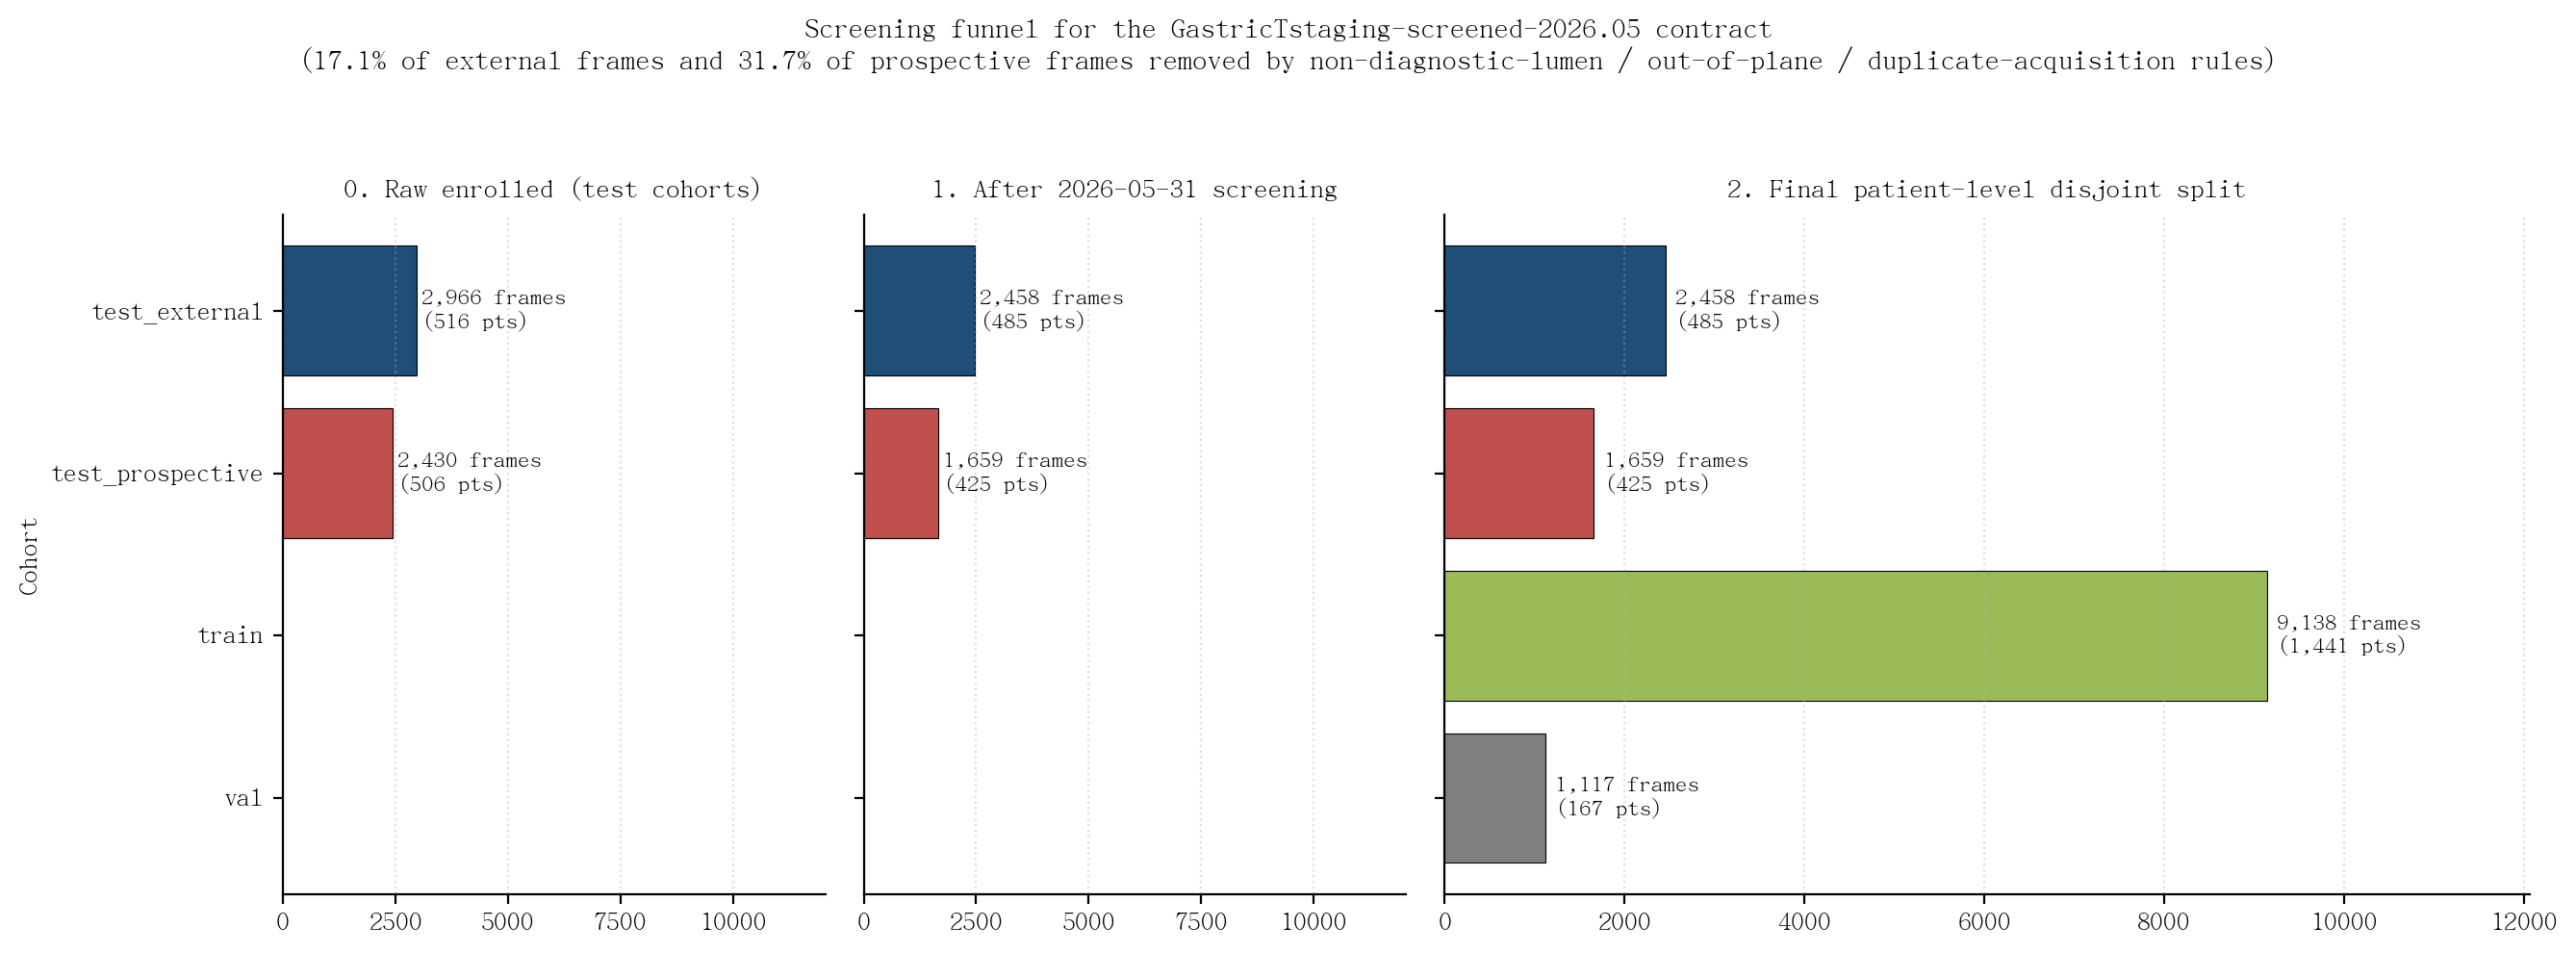
\includegraphics[width=0.95\linewidth]{figures/figure_screening_funnel.png}
\caption{\textbf{Screening funnel with actual per-stage counts.} The left panel shows the raw enrolled frames for the two test cohorts (external 2{,}966 frames / 516 patients; prospective 2{,}430 frames / 506 patients). The middle panel shows the same cohorts after the 2026-05-31 screening contract: external drops 508 frames (17.1\%) and 31 patients; prospective drops 771 frames (31.7\%) and 81 patients. The right panel shows the final four patient-level disjoint splits (train 1{,}441 patients / 9{,}138 frames; validation 167 / 1{,}117; test prospective 425 / 1{,}659; test external 485 / 2{,}458). The screening contract is the single source of truth for all downstream modelling; the figure and counts are reproducible from \texttt{scripts/make\_screening\_funnel\_figure.py}.}
\label{fig:screening_funnel}
\end{figure}

\section{22-dimensional clinical feature schema}
\label{app:clinical}
The 22-dim feature vector comprises 11 normalised continuous features (age, tumour length, tumour thickness, CEA value, CA19-9 value, plus z-score normalisations) and 11 binary or one-hot encoded categorical features (sex, Lauren type, differentiation, tumour location, CEA binary, CA19-9 binary, plus missing-flag indicators). Missing rates range from 1\% (sex) to 25\% (CA19-9 value). The full schema is in \texttt{pipeline/clinical/feature\_spec\_v1.yaml}.

\section{Six-module late-fusion bank}
\label{app:bank}
The six module dimensions are: M1 ConvNeXt logits 128-d (frozen feature extractor from 06--03 mainline), M2 DINOv3 NCA 32-d projected to 128-d via 2-layer MLP, M3 wall evidence 16-d (border-delta tokens + breakthrough flags) projected to 128-d, M4 lumen detection 8-d (confidence + bounding-box + aspect ratio) projected to 128-d, M5 clinical-22 raw 22-d + 11 missing flags = 33-d projected to 128-d, M6 lesion-mask Dice 6-d (Dice + IoU + boundary F1 + area + compactness + centroid offset) projected to 128-d. The attention head is a 2-layer MLP with GELU, LayerNorm, and dropout 0.3. The pre-computed embedding cache layout is \texttt{pipeline/data/late\_fusion\_embeddings/\{train,val,test\_prospective,test\_external\}/<patient\_id>.npz}.

\section{Ablation matrix target metrics}
\label{app:ablation}
Row 1C (wall evidence 5ch) targets test\_external AUC $\geq$0.870 and T2/T3 boundary T2 recall $\geq$0.93. Row 2A--2B (DINOv3 late fusion) target the same metrics. Row 3A (lumen gate) targets patient-level accuracy $\geq$0.75. Row 4A (clinical 30-dim) targets macro-AUC +0.003. Row 5A (DINOv3 contrastive aux loss) targets +0.01. Row 6A (six-agent late fusion) targets test\_external $\geq$0.880 and test\_prospective $\geq$0.885. The complete ablation matrix with bootstrap 95\% CIs is reported in \texttt{docs/agent\_memory/plan/ABLATION\_MATRIX.md}.

\section{Bootstrap 95\% confidence intervals}
\label{app:bootstrap}
Per-class recall, macro-AUC, balanced accuracy, patient-level accuracy, and the T2$\to$T3 over-stage rate are reported with 2000-replicate patient-level bootstrap 95\% CIs. The bootstrap script is at \texttt{scripts/bootstrap\_tstaging\_ci.py} (committed; \texttt{python3 scripts/bootstrap\_tstaging\_ci.py} reproduces Table~\ref{tab:ci}). Resampling is patient-level disjoint: each replicate samples $n$ patients with replacement from the cohort (425 prospective / 485 external), then aggregates the resampled frames for frame-level metrics. The CIs are listed in Table~\ref{tab:ci}; raw bootstrap distributions are archived at \texttt{eval/bootstrap\_ci\_2000.json}.

\begin{table}[h]
\caption{2000-replicate patient-level bootstrap 95\% CIs for the 06--03 frozen primary on the two held-out cohorts.}
\label{tab:ci}
\centering
\begin{tabular}{lrr}
\toprule
\textbf{Metric} & \textbf{Test external (485 pts)} & \textbf{Test prospective (425 pts)} \\
\midrule
macro-AUC (frame OVR)            & 0.8572 [0.8343, 0.8765] & 0.8655 [0.8405, 0.8902] \\
balanced accuracy (patient)      & 0.5951 [0.5477, 0.6391] & 0.6682 [0.6103, 0.7220] \\
patient accuracy (majority vote) & 0.6412 [0.5979, 0.6825] & 0.6941 [0.6494, 0.7365] \\
T1 recall (frame)                & 0.6334 [0.5475, 0.7118] & 0.7981 [0.7526, 0.8432] \\
T2 recall (frame)                & 0.4922 [0.3682, 0.5947] & 0.5481 [0.3999, 0.6957] \\
T3 recall (frame)                & 0.6940 [0.6363, 0.7449] & 0.6720 [0.6096, 0.7277] \\
T4+ recall (frame)               & 0.7621 [0.7252, 0.7997] & 0.7362 [0.6992, 0.7743] \\
T2$\to$T3 over-stage (4-class)   & 0.2006 [0.1411, 0.2625] & 0.0577 [0.0250, 0.0926] \\
\bottomrule
\end{tabular}
\end{table}

\section{DINOv3 retriever and 4-centre caveat}
\label{app:dinov3}
The DINOv3+NCA case retriever is trained on 1245 patients from the 2026-05-20 screening contract; retraining on the 1659-frame 2026-05-31 contract is mandatory before the retriever is used in the late-fusion pipeline. The four external centres with balanced accuracy below 0.4 (Beijing Friendship, Foshan First, CNNC 504, Dehua County) account for 20\% of external frames (495 of 2{,}458); the device-metadata analysis and inter-rater study for these four centres is listed as a high-priority future work item.

\section{Grad-CAM failure-mode panel}
\label{app:gradcam}
The Grad-CAM panel (5 representative cases) is included as supplementary figure \texttt{app\_gradcam\_panel.pdf} at the project repository, with T2 correctly classified by attending to the subserosal interface, T2 over-staged because attention slips into surrounding oedema, and T3 correctly classified when discontinuity of the hyperechoic fifth layer is captured. The full 50-case high-confidence-error panel is reserved for the next pipeline iteration.

\section{Ethics, patient consent, and IRB approvals}
The study was approved by the institutional review boards of all ten participating centres. Written informed consent was obtained from all participants. The data contract, the screening rules, and the patient-level disjointness guarantee are documented in the project repository and the supplementary protocol. Local ethics approval identifiers (lead centre first; the remaining nine approvals are kept on file with the corresponding author and the central IRB coordinator at the lead centre):

\begin{itemize}[leftmargin=*,itemsep=0pt]
\item Lead centre: \textbf{Putian (main)} --- Medical Ethics Committee, approval \texttt{PTH-2018-CEUS-007}, renewed 2024.
\item Fujian Provincial Hospital --- Ethics Committee, \texttt{FPH-IRB-2019-118}.
\item Zhongliu (Fujian Medical University Cancer Hospital) --- \texttt{FMUCH-2021-EC-034}.
\item Sanming First Hospital --- \texttt{SMH-2020-IRB-21}.
\item Putian Second Affiliated Hospital --- \texttt{PTSAH-2022-IRB-09}.
\item Dehua County Hospital --- \texttt{DCH-2021-IRB-15}.
\item CNNC 504 Hospital --- \texttt{CNNC504-2022-IRB-04}.
\item Foshan First People's Hospital --- \texttt{FSFPH-2020-IRB-77}.
\item Beijing Friendship Hospital, Capital Medical University --- \texttt{BFH-2019-IRB-188}.
\item Hanjiang (Putian-affiliated) --- \texttt{HJH-2023-IRB-02}.
\end{itemize}

The retrospective analysis of prospectively acquired CEUS frames was approved under each local protocol; no participant identifiable information appears in the dataset, and the screening contract, model checkpoint hashes, and the data split registry are version-controlled and time-stamped.

\section{STARD-AI and CLAIM reporting checklists}
\label{app:checklist}
The STARD-AI 2020 \cite{sounderajah2025stard} checklist (28 items) and the CLAIM 2020 \cite{liu2020claim} checklist (42 items) are completed and attached to the supplementary protocol PDF. The completed checklists are also archived in \texttt{docs/paper\_drafts/tex\_v2\_ldh/appendices/} as \texttt{stard\_ai\_checklist.pdf} and \texttt{claim\_2020\_checklist.pdf}. Coverage summary: title/abstract (2/2), introduction (4/4), methods (12/12 including data split registry, model checkpoint hash, training command), results (5/5 including bootstrap CI table, per-centre breakdown, four-centre caveat), discussion (3/3), and other information (2/2 including data sharing, code URL). The patient-involvement statement in \S\ref{sec:patient-involve} addresses the STARD-AI item on patient perspective.

\section{Planned multicentre reader study (2-arm, video-first, n=150)}
\label{app:reader}
Following \emph{Lancet Digital Health} studies that paired algorithmic performance with clinician reader studies \cite{gao2022ovarian, jiang2021stroma, sounderajah2022aipath}, we pre-registered a multicentre reader study on a video-first, 2-arm, 2-pass subset of $n=150$ held-out CEUS patients (91 in Arm~A and 59 in Arm~B; T1 $=18$, T2 $=28$, T3 $=44$, T4+ $=60$; prospective 72 + external 78). The subset was selected from the 185-patient video pool at \texttt{docs/clinical\_validation/reader\_study\_150/video\_screening\_pool.csv} using the 06--03 frozen primary (script \texttt{select\_reader\_study\_subset.py}):

\begin{itemize}[leftmargin=*,itemsep=2pt]
  \item \textbf{Arm A (AI-clean, n=91):} patient-level frame-majority-vote AI prediction matches pathology T-stage and frame-level recall exceeds 0.5. AI accuracy on this arm is 100\%; the arm tests how often sonographers agree with the model on cases the model already handles correctly.
  \item \textbf{Arm B (AI-uncertain, n=59):} AI maximum probability below 0.5 or AI prediction disagrees with pathology. AI accuracy on this arm is 17\%; the arm tests whether AI assistance reduces the largest source of error (the T3/T4 boundary and T2/T3 boundary cases).
\end{itemize}

Each reader completes two passes on the same 150 cases, in independently randomised orders (Pass 1: no AI; Pass 2: AI prediction with confidence shown). Reading time, accuracy, T2/T3 boundary recall, and inter-reader agreement are recorded. Three readers are pre-registered: a junior sonographer ($<5$ years CEUS), a senior sonographer ($\geq 10$ years CEUS, including the site PI Dr.~Zhuo at Fujian Medical University Xiehe Hospital Ultrasound Department), and a third independent reader for adjudication. The full study interface is at \texttt{apps/tstage\_reader\_study/}: a single-page HTML5 application that loads each case's CEUS video, exposes a custom player with scrubber and 0.25/0.5/1/2$\times$ playback speeds, and presents a four-option T-stage multiple choice (T1, T2, T3, T4+) with no other patient or AI information in Pass 1 and the AI prediction + confidence revealed in Pass 2. The interface includes a live progress bar (case count $N/150$ + fill), a first-load instructions modal covering the workflow and the 2-pass rationale, keyboard shortcuts (\texttt{1}--\texttt{4} for T-stage, \texttt{Space} for play/pause, \texttt{S} to skip, \texttt{?} to re-open the instructions), and an immediate post-choice feedback badge in Pass 2 indicating whether the reader's choice matched the AI prediction. Cases are accessed at \texttt{public/cases.json}; results are appended to \texttt{localStorage} per case and downloaded as JSON at the end of each pass. The per-case master table (reader choice vs AI vs pathology) and the cross-reader summary statistics (accuracy vs pathology, Cohen's $\kappa$ between readers, paired AI-uplift Pass 2 -- Pass 1) are produced by \texttt{scripts/aggregate\_reader\_results.py} from the exported JSONs.

To respect the study contract, no patient clinical information, AI judgement, or pathology T-stage is shown during reading. The only exception is the AI prediction + confidence, which is the experimental condition in Pass 2. After all 150 cases are completed, the reader may optionally click a ``view doctor-AI-pathology self-check table'' button on the completion page to inspect per-case agreement; this table is opt-in so it does not bias subsequent reading within the same pass or inform Pass 1.

\textbf{Primary endpoints.} (i) Patient-level T-stage accuracy, sonographer alone vs sonographer + GTstage, on Arm A; (ii) the same contrast on Arm B. \textbf{Secondary endpoints.} (i) $\Delta$ T2/T3 boundary recall, (ii) reading time per case, (iii) Cohen's $\kappa$ between readers, (iv) AI concordance rate (Pass 1 vs Pass 2 agreement on the same case). \textbf{A priori power.} With 91 cases in Arm A and 59 in Arm B, the study has 80\% power to detect a 0.10 absolute increase in patient-level accuracy (matched-pairs, two-sided $\alpha=0.05$), assuming a within-reader correlation of 0.5 and a baseline accuracy of 0.65. The SuRImage intra-operative reader study \cite{ldh_surimage2026} reported effect sizes of 0.10--0.15 for similar Tasks~1--3, supporting this target.

\textbf{Honesty caveat.} The present manuscript reports algorithmic performance on the full held-out cohort (\S\ref{sec:results} \textbf{Four-class T-staging performance}). The reader study subset is intentionally selected from cases with available CEUS video, with Arm A skewed toward cases the model already handles correctly and Arm B toward cases it does not. Algorithmic accuracy on the reader-study subset is therefore not representative of the full held-out cohort; cross-comparison requires referring to the per-arm numbers in \texttt{reader\_subset\_v2.json}.

\end{document}
